\documentclass{article}
\usepackage{amssymb}
\usepackage{amsmath}
\usepackage{graphicx}
\usepackage{subfigure}
\usepackage[margin=1in]{geometry}
\author{Tianyu Dai, Xiaoqing Li, Xuejian Ma, Yuheng Liao }
\title{PHY566 - Diffusion Equation}
\begin{document}
\date{3/22/2017}
\maketitle
\section{Problem 1}
\quad To solve this problem, we first consider one random walker and get its $x_{n}$. Put a
random walker at the origin. Create a random number $movestep$ in range
(0,1,2,3), and these four numbers means moving one step right/left/up/down
respectively.

We create a zero list to record the number of moving steps in every
direction. After we know the moving direction of a step, we add 1 to the number of
total steps in that certain direction. If the total number of moving
steps is $n$, we repeat the previous procedure $n$ times. The number of
total rightward steps minus the number of total leftward steps generates the
x-component of the random walker's displacement, $x_{n}$. Likewise, the
number of total upward steps minus the number of total downward steps
generates the y-component of the random walker's displacement, $y_{n}$.

After that, $x_{n}^{2}$ and $r_{n}^{2}$ are easy to calculate. We use a
function named random\_walk to return the values of $x_{n}$,  $x_{n}^{2}$,
and $r_{n}^{2}$. Since our goal is averaging over $10^{4}$ different
walkers, we need a loop with $10^{4}$ iterations to get the values of $%
x_{n}$, $x_{n}^{2}$, and $r_{n}^{2}$ of each walker, and then realize the
average values, $\left\langle x_{n}\right\rangle $, $\left\langle
x_{n}^{2}\right\rangle $, and $\left\langle r_{n}^{2}\right\rangle $.
\begin{figure}[!ht]
	\centering
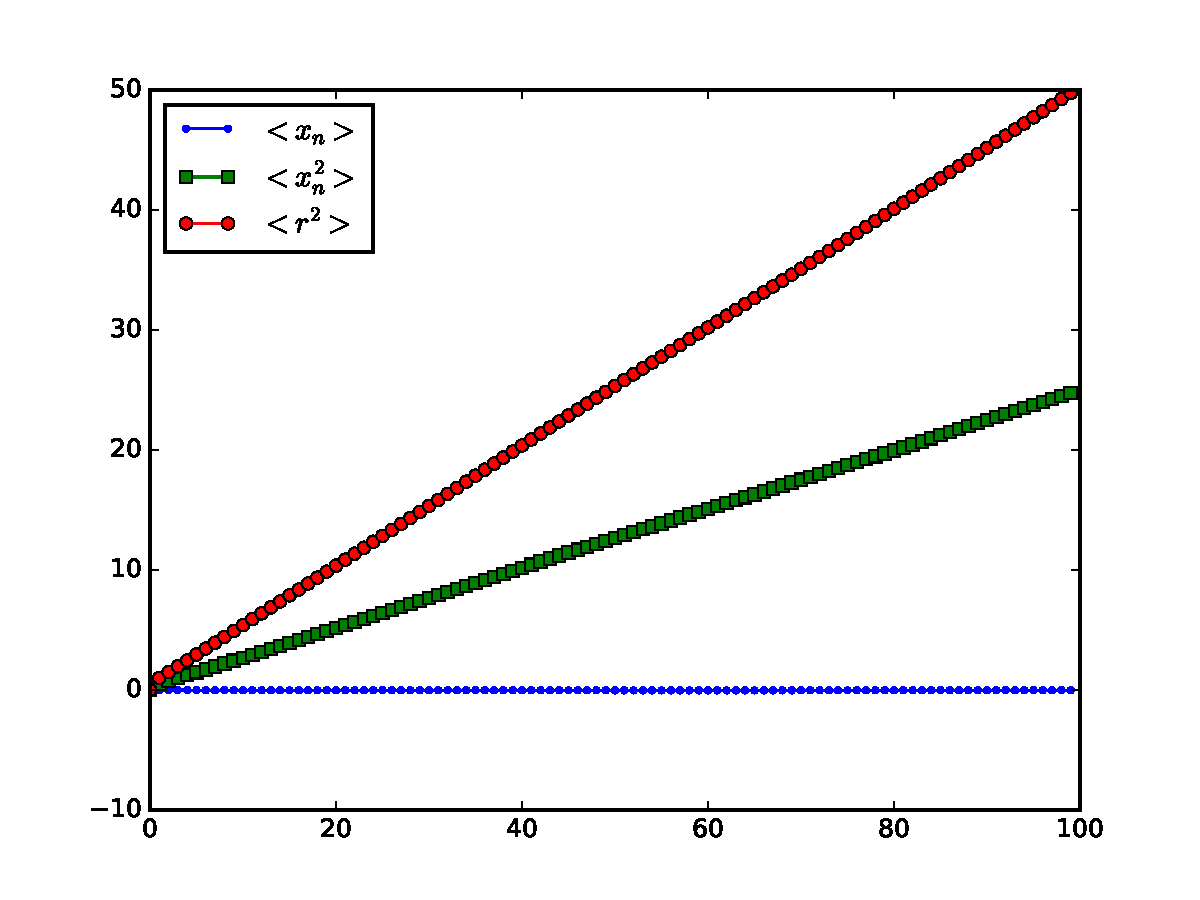
\includegraphics[width=0.8\textwidth]{./RandomWalk.pdf}
\end{figure}
\section{Problem 2}
\subsection{Part A}
\quad To calculate $\left<x(t)^2\right>$, we can integrate it by part:
\begin{eqnarray}
% \nonumber % Remove numbering (before each equation)
  \nonumber \rho(x,t) &=& \frac{1}{\sqrt{2\pi \sigma(t)^2}}exp\left(-\frac{x^2}{2\sigma (t)^2}\right) \\
  \nonumber \left<x(t)^2\right> &=& \int_{-\infty}^{\infty} x^2\frac{1}{\sqrt{2\pi \sigma(t)^2}}exp\left(-\frac{x^2}{2\sigma (t)^2}\right)dx \\
  \nonumber \left<x(t)^2\right> &=& \int_{-\infty}^{\infty} \sigma(t)^2x\frac{1}{\sqrt{2\pi \sigma(t)^2}}d\left(\exp{\frac{-x^2}{2\sigma (t)^2}}\right)  \\
  \nonumber \left<x(t)^2\right> &=& \sigma(t)^2\int_{-\infty}^{\infty} \frac{1}{\sqrt{2\pi \sigma(t)^2}}exp\left(-\frac{x^2}{2\sigma (t)^2}\right)dx  \\
  \nonumber \left<x(t)^2\right> &=& \sigma(t)^2
\end{eqnarray}
\quad Therefore,the spatial expectation value $\left<x(t)^2\right>$ of the 1D Normal Distribution equals $\sigma(t)^2$
\subsection{Part B}
\quad The diffusion equation is:
\begin{eqnarray}
% \nonumber % Remove numbering (before each equation)
  \nonumber \frac{\partial\phi(\vec r, t)}{\partial t} &=& D\nabla^2 \phi(\vec r, t)
\end{eqnarray}
\quad where $D=2$ is a diffusion constant.

For a linear diffusion equation:
\begin{eqnarray}
% \nonumber % Remove numbering (before each equation)
  \nonumber \frac{\partial\phi(\vec r, t)}{\partial t} &=& D\frac{d^2\phi(\vec r, t)}{dx^2}
\end{eqnarray}
\quad The numerical solution is:
\begin{eqnarray}
% \nonumber % Remove numbering (before each equation)
  \nonumber \frac{y_{j+1, i}-y_{j, i}}{\Delta t} &=& D\frac{y_{j, i+1}+y_{j, i-1}-2y_{j, i}}{\Delta x^2} \\
  \nonumber y_{j+1, i} &=& y_{i, j}+\frac{D\Delta t}{\Delta x^2}(y_{j, i+1}+y_{j, i-1}-2y_{j, i})
\end{eqnarray}
\quad After getting y in each x for each time snapshot, we obtained $\sigma(t)$ by fitting it into equation:
\begin{eqnarray}
% \nonumber % Remove numbering (before each equation)
  \nonumber \rho(x,t) &=& \frac{1}{\sqrt{2\pi \sigma(t)^2}}exp\left(-\frac{x^2}{2\sigma (t)^2}\right)
\end{eqnarray}
\quad We choose 5 time snapshots [1,50,120,200,280]($\Delta t=0.01$) to get $\sigma(t)$ and plot them in following figure.
\begin{center}
  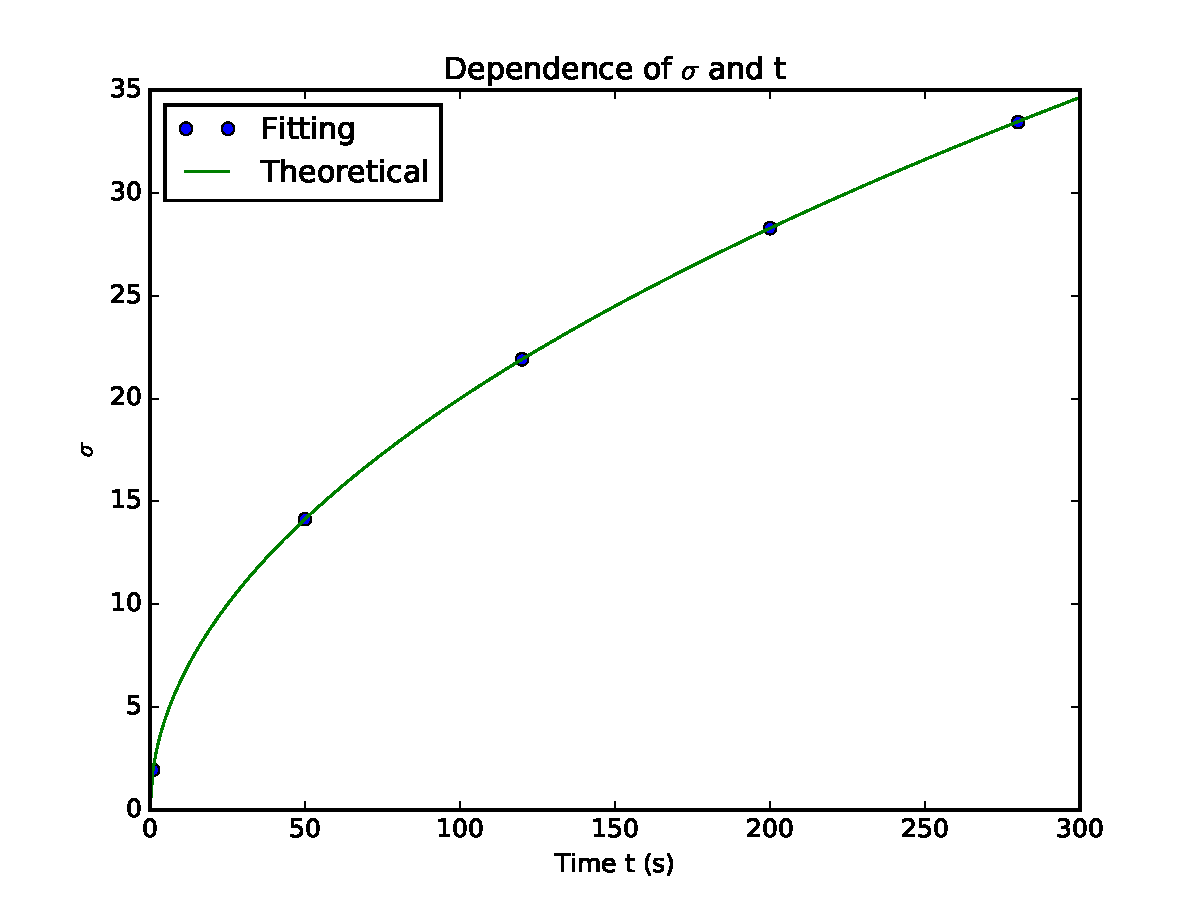
\includegraphics[width=0.8\textwidth]{./sigma.pdf}
\end{center}
\quad The fitting points match the analytical function perfectly.
\section{Problem 3}
\subsection{Part A}
\quad First, we set up the initial condition by generating a matrix with $80$ rows
and $120$ columns and assigning $-1$ and $1$ to the first $40$ columns and
the last $40$ columns respectively. Here, $-1$ means this site is occupied
by a A-molecule, and $1$ means it is occupied by a B-molecule. We also
generate a matrix with $2\times N$ rows and $2$ columns, where $N$
represents the number of molecules of each species.

The first and second half $80\times 40$ rows respectively record the coordinates of A molecules
and B molecules. For every step, we generate a random number to decide which
molecule to move in which direction. Since there are $2\times N$ molecules
and every molecule can move in up/down/left/right four different directions,
we have to pick a random number, $R$, from the range $\left[ 0,2\times
N\times 4-1\right] $. $m=R\%(2N)$ means the molecule decided by the random
number $R$, and $move=R/(2N)$ means the moving direction decided by $R$. We
can extract the coordinates of the molecule as $x=mol[m,0]$, and $y=mol[m,1]$%
. The next step is moving the picked molecule. $move=0,1,2,3$ means the
moving direction is up/down/left/right, respectively.

 However, this grid has
boundary. Specifically, a molecule on the upper side cannot move upward, a
molecule on the lower side cannot move downward, a molecule on the left side
cannot move leftward, and a molecule on the right side cannot move
rightward. If $move=0$, $y$ cannot be $79$, and we demand $y+1<80$. Then, if
$sites[y+1,x]=0$, it means the site right above this molecule is not
occupied and we can move the molecule to that site. After the movement, we update the distribution on the grid by assigning the value
of $sites[y,x]$ to $sites[y+1,x]$ and assigning $0$ to $sites[y,x]$, then update the molecule's coordinates by adding 1 to its
y-coordinate. If $%
move=1$, $y$ cannot be $0$, and we demand $y-1>0$, and if $sites[y-1,x]=0$,
we move the molecule one step down and update its coordinates and the
distribution. For $m=1$ and $m=2$, the procedure is the same.

\subsection{Part b}
\quad To plot the linear population densities $n_{A}(x)$ and $n_{B}(x)$, we need
to know there are how many A-molecules and B-molecules on each column
respectively. We use a nested loop to complete this job, the inner one is to
count there are how many $1$ and $-1$ on each column respectively. The
number of $1$ means the number of B-molecules, and the number of $-1$ means
the number of A-molecules. Then record the values in two lists maned sumA
and sumB. For example, if a loop is running for the $i^{th}$ column, sumA[i]
is the number of A-molecules on the $i^{th}$ column, and sumB[i] is the
number of B-molecules on this column. The outer loop makes the inner one
runs for each column. Finally, divide sumA[i] and sumB[i] by the length of
the left or right side, $80.0$, we obtain the linear population densities $%
n_{A}(x)$ and $n_{B}(x)$. The distribution figures and the density figures
of the two gases on the grid are shown below. Here, we plot the matrix, $%
sites$, with imshow to generate the distribution figures.
\begin{figure}[!ht]
	\centering
	\subfigure{
		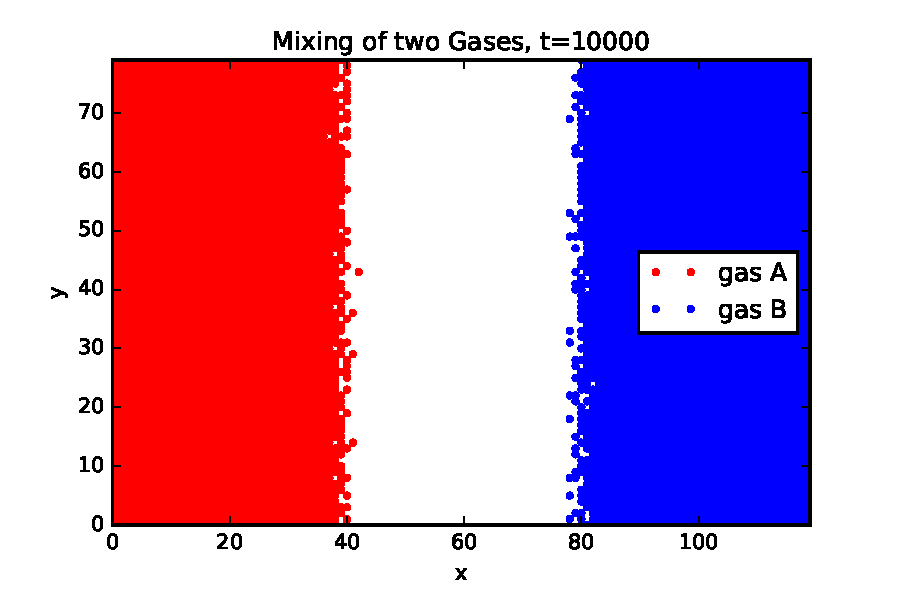
\includegraphics[width=.8\columnwidth]{mixing_1.pdf}
	}
	\subfigure{
		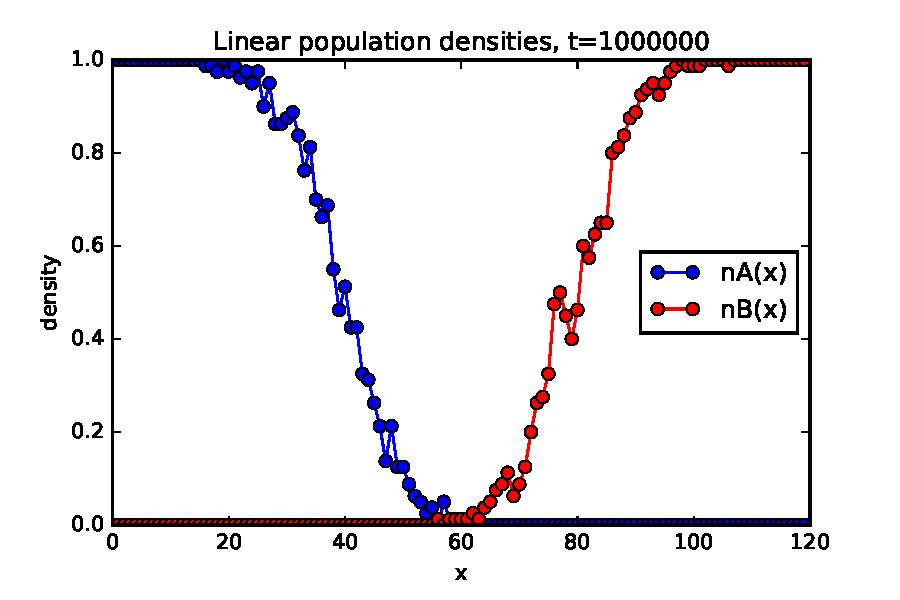
\includegraphics[width=.8\columnwidth]{densities_1.pdf}
	}
\end{figure}
\begin{figure}[!ht]
	\centering
	\subfigure{
		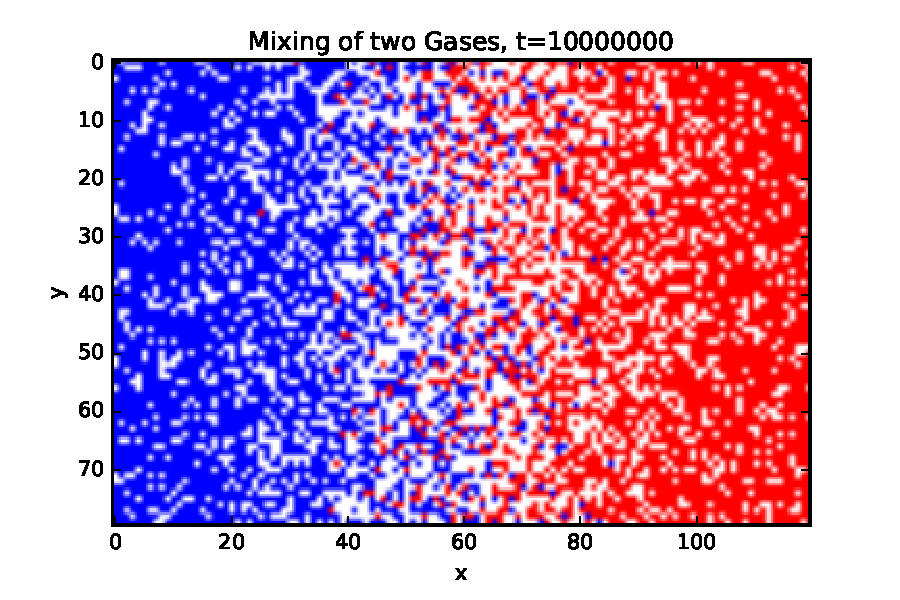
\includegraphics[width=.8\columnwidth]{mixing_2.pdf}
	}
	\subfigure{
		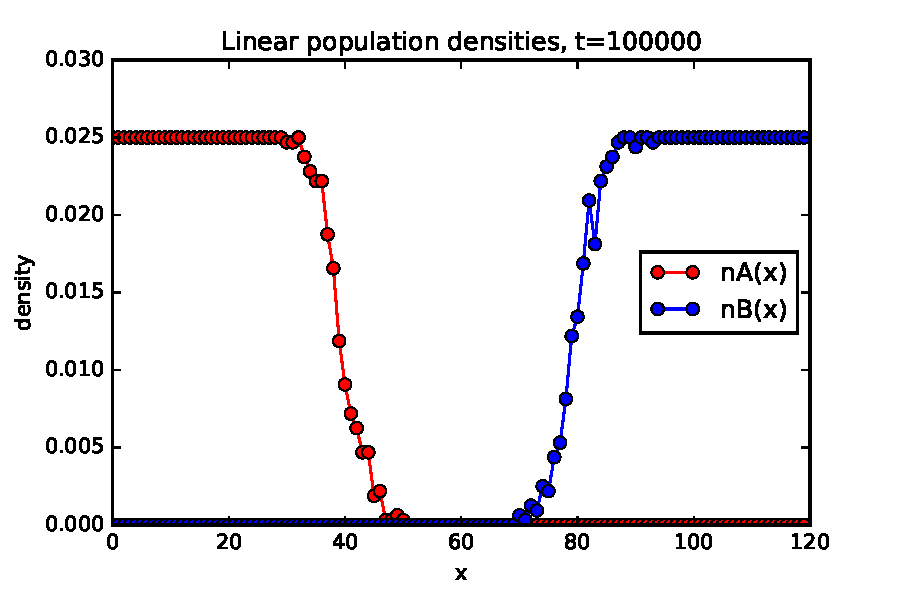
\includegraphics[width=.8\columnwidth]{densities_2.pdf}
	}
\end{figure}
\begin{figure}[!ht]
	\centering
	\subfigure{
		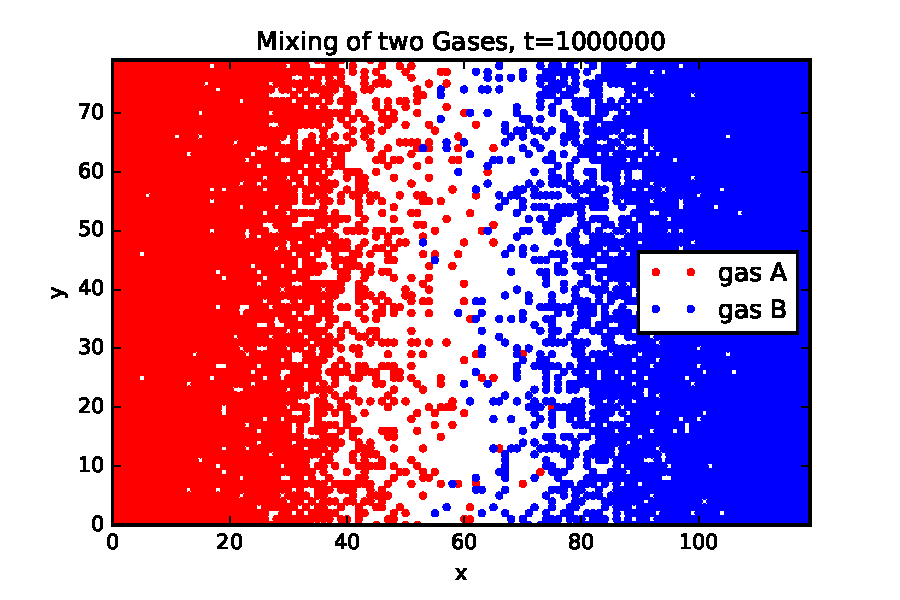
\includegraphics[width=.8\columnwidth]{mixing_3.pdf}
	}
	\subfigure{
		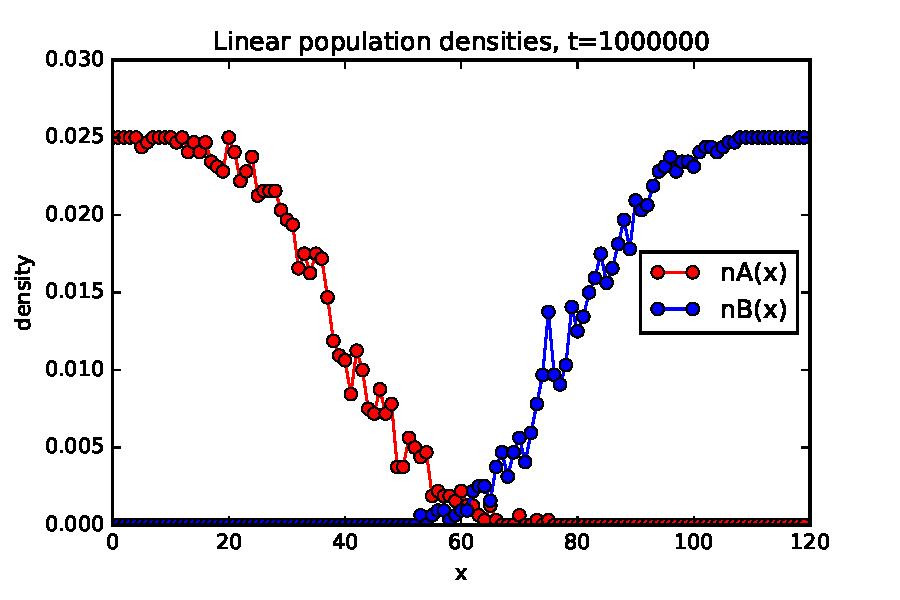
\includegraphics[width=.8\columnwidth]{densities_3.pdf}
	}
\end{figure}
\begin{figure}[!ht]
	\centering
	\subfigure{
		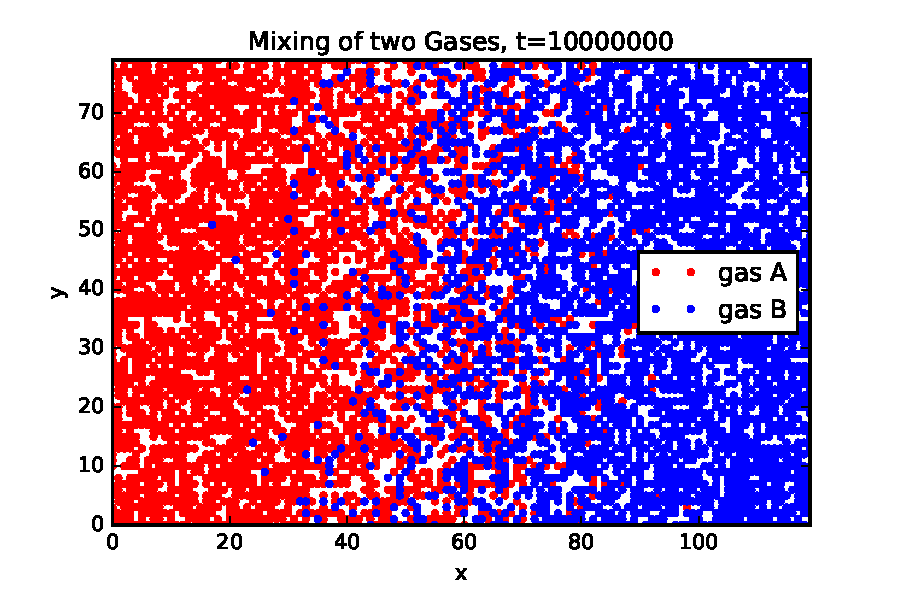
\includegraphics[width=.8\columnwidth]{mixing_4.pdf}
	}
	\subfigure{
		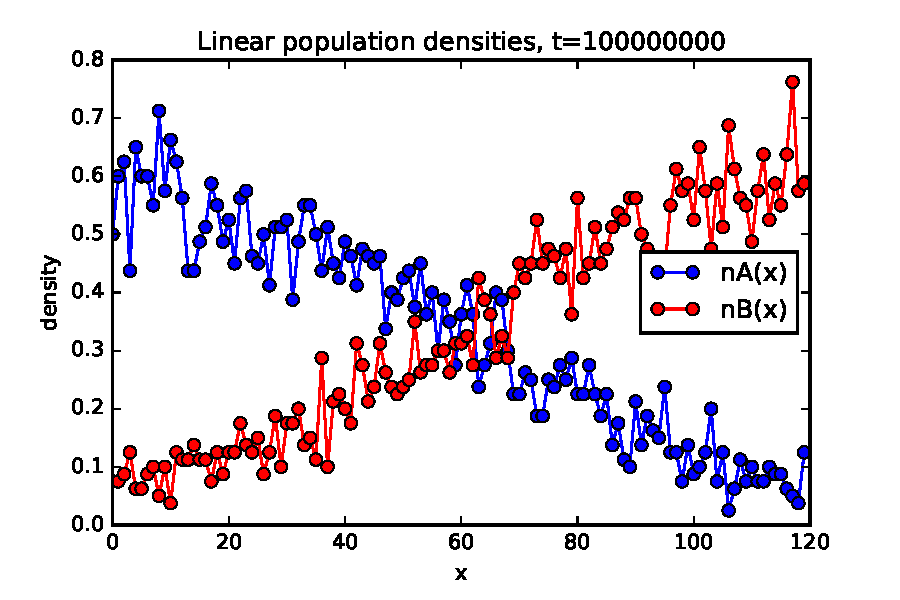
\includegraphics[width=.8\columnwidth]{densities_4.pdf}
	}
\end{figure}
\begin{figure}[!ht]
	\centering
	\subfigure{
		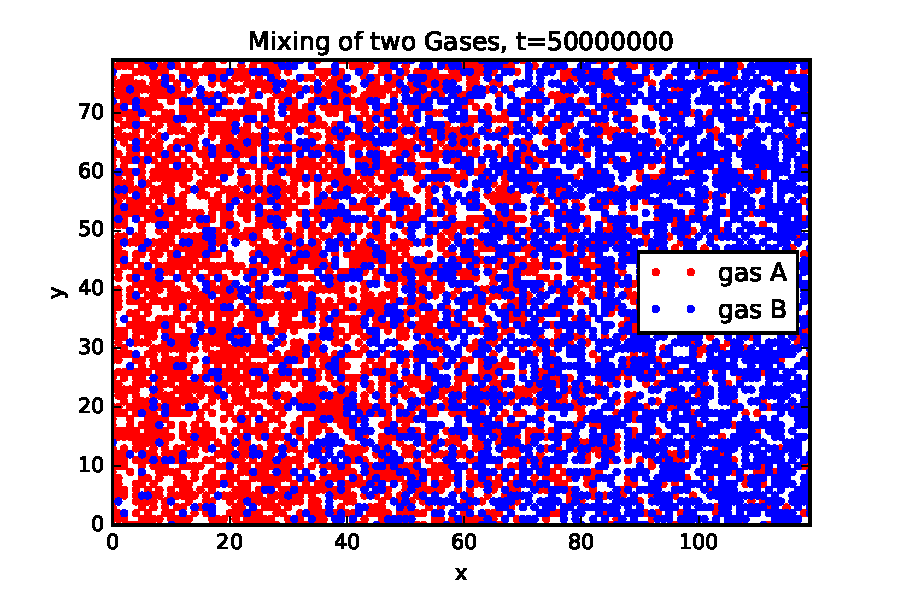
\includegraphics[width=.8\columnwidth]{mixing_5.pdf}
	}
	\subfigure{
		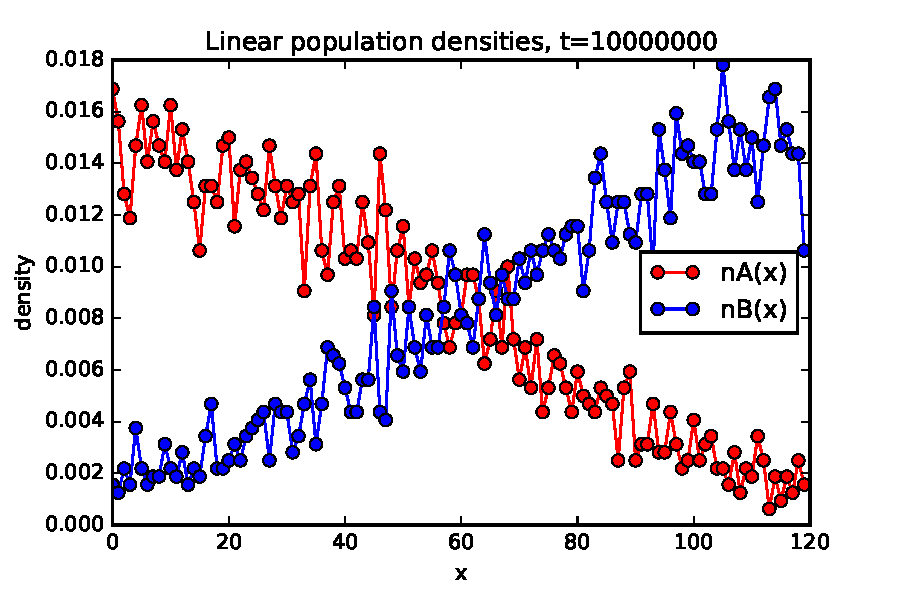
\includegraphics[width=.8\columnwidth]{densities_5.pdf}
	}
\end{figure}
\begin{figure}[!ht]
	\centering
	\subfigure{
		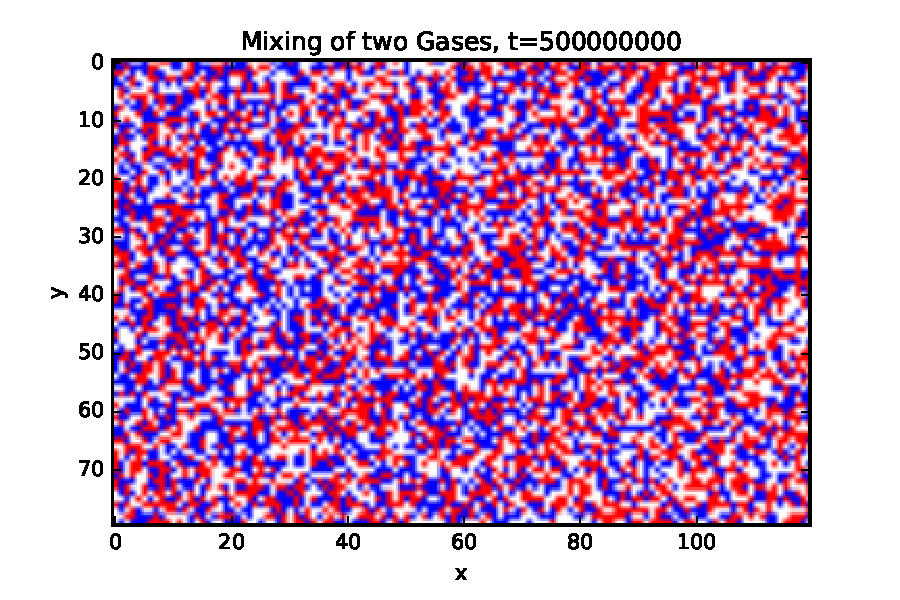
\includegraphics[width=.8\columnwidth]{mixing_6.pdf}
	}
	\subfigure{
		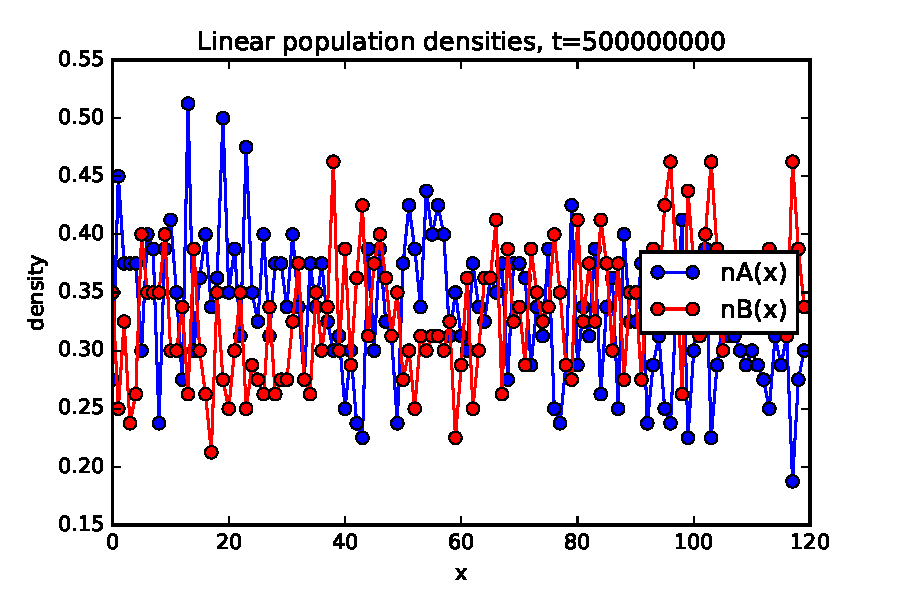
\includegraphics[width=.8\columnwidth]{densities_6.pdf}
	}
\end{figure}
\clearpage
\subsection{Part C}
\quad To average the densities over 100 trials for added accuracy, we only need a bigger loop outside the program of part (b) to run the code 100 times, and then average them. We make a comparison of linear population densities between one trial and the average of 100 trials as the following.
\begin{figure}[!ht]
	\centering
	\subfigure{
		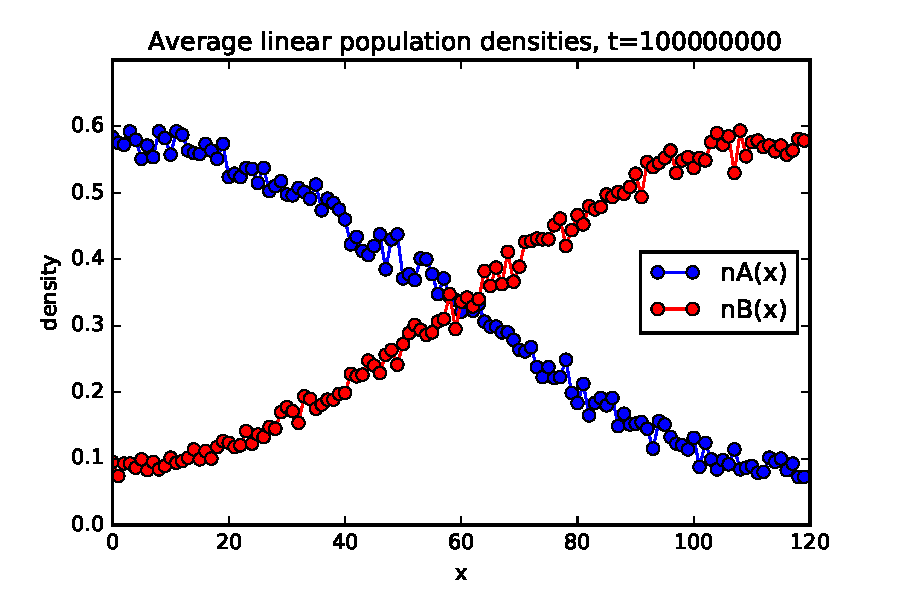
\includegraphics[width=.8\columnwidth]{average_densities.pdf}
	}
	\subfigure{
		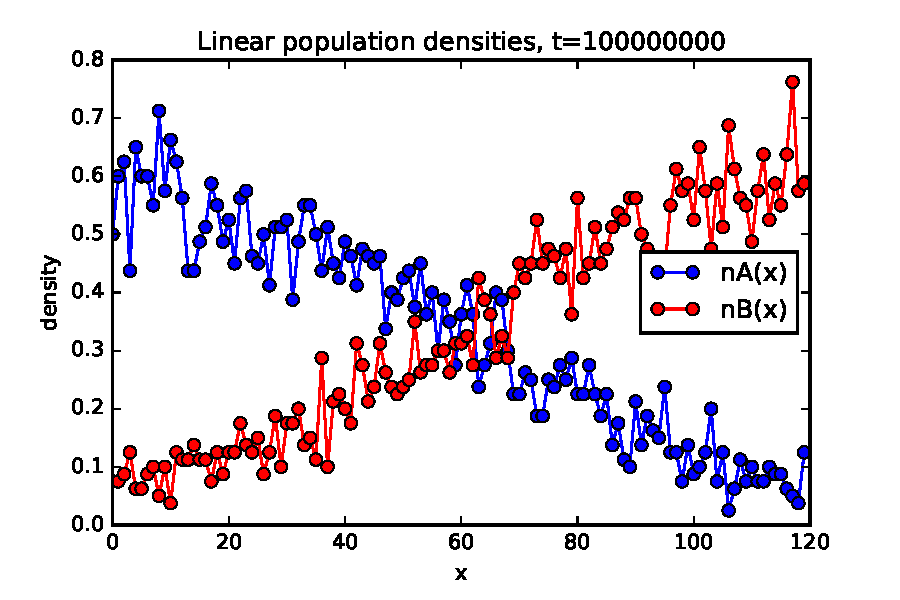
\includegraphics[width=.8\columnwidth]{densities_4.pdf}
	}
\end{figure}

\end{document}
